
\documentclass[tikz,border=2mm]{standalone}
\usepackage[utf8]{inputenc}
\usepackage[T1]{fontenc}
\usepackage{amsmath}
\usepackage{amssymb}
\usetikzlibrary{arrows.meta,positioning,calc,shapes.geometric}
\usepackage{xcolor}

\definecolor{inkNavy}{HTML}{1B2733}
\definecolor{slate}{HTML}{3B4B5C}
\definecolor{paper}{HTML}{FBFAF7}
\definecolor{amber}{HTML}{C97A2B}
\definecolor{teal}{HTML}{2E7D74}
\definecolor{softred}{HTML}{A6402F}
\definecolor{lightgrey}{HTML}{E7E4DD}
\definecolor{midgrey}{HTML}{8B8A85}

\begin{document}
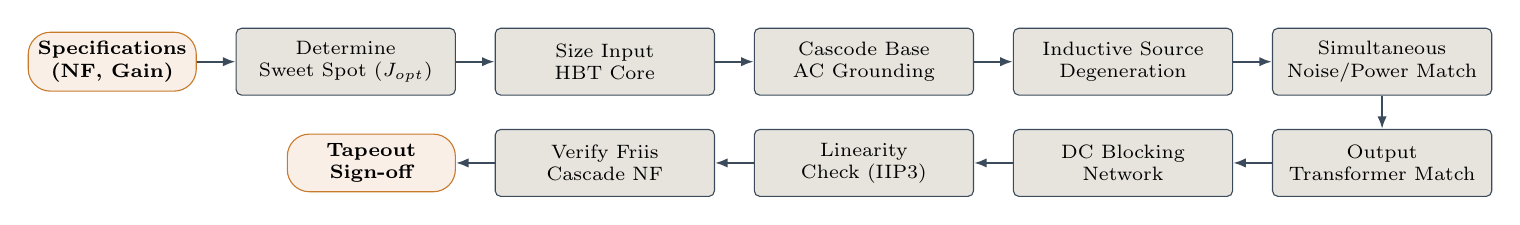
\begin{tikzpicture}[
  node distance=6pt and 14pt,
  box/.style={draw=slate, fill=lightgrey, rounded corners=2pt, text width=2.55cm, align=center, minimum height=0.85cm, font=\scriptsize},
  term/.style={draw=amber, fill=amber!12, rounded corners=8pt, text width=1.9cm, align=center, minimum height=0.7cm, font=\scriptsize\bfseries},
  arr/.style={-{Latex[length=1.6mm]}, slate, thick}
]
\node[term] (spec) {Specifications\\(NF, Gain)};
\node[box, right=of spec] (jopt) {Determine\\Sweet Spot ($J_{opt}$)};
\node[box, right=of jopt] (size) {Size Input\\HBT Core};
\node[box, right=of size] (casc) {Cascode Base\\AC Grounding};
\node[box, right=of casc] (degen) {Inductive Source\\Degeneration};
\node[box, right=of degen] (snpm) {Simultaneous\\Noise/Power Match};

\node[box, below=12pt of snpm] (out) {Output\\Transformer Match};
\node[box, left=of out] (block) {DC Blocking\\Network};
\node[box, left=of block] (iip3) {Linearity\\Check (IIP3)};
\node[box, left=of iip3] (pvt) {Verify Friis\\Cascade NF};
\node[term, left=of pvt] (fin) {Tapeout\\Sign-off};

\draw[arr] (spec)--(jopt); \draw[arr] (jopt)--(size); \draw[arr] (size)--(casc);
\draw[arr] (casc)--(degen); \draw[arr] (degen)--(snpm); \draw[arr] (snpm)--(out);
\draw[arr] (out)--(block); \draw[arr] (block)--(iip3); \draw[arr] (iip3)--(pvt);
\draw[arr] (pvt)--(fin);
\end{tikzpicture}
\end{document}